% !TEX program = xelatex
% Compile: xelatex squeezing_report_v6.tex  (run twice for references)
% Figures:
%   squeezing_frontier_v6.png
%   squeezing_frontier_od_v6.png
%   squeezing_frontier_hardened_compare_v6.png
%   squeezing_frontier_ideal_qe1_v6.png
%   squeezing_frontier_ideal_v6_tpd_angle_detail.png
%   squeezing_frontier_ideal_v6_low_angle_ridge.png
\documentclass[11pt,a4paper]{article}

\usepackage{kotex}
\setmainhangulfont{Malgun Gothic}
\setsanshangulfont{Malgun Gothic}

\usepackage{amsmath,amssymb}
\usepackage{graphicx}
\usepackage{booktabs}
\usepackage{array}
\usepackage{tabularx}
\usepackage{geometry}
\geometry{margin=2.4cm}
\usepackage{caption}
\captionsetup{font=small,labelfont=bf}
\usepackage{enumitem}
\usepackage{xcolor}
\usepackage[hidelinks]{hyperref}
\graphicspath{{./}}
\sloppy

\newcommand{\dB}{\,\mathrm{dB}}
\newcommand{\GHz}{\,\mathrm{GHz}}
\newcommand{\MHz}{\,\mathrm{MHz}}
\newcommand{\degC}{\,^{\circ}\mathrm{C}}

\title{\textbf{$^{85}$Rb D1 이중-$\Lambda$ 사파장혼합(FWM) 트윈빔\\
세기차 스퀴징 최적점 재분석}\\[3pt]
\large 보고서 v6: seeded beat 부호 교정 이후의 frontier와 TPD/angle 진단}
\author{GABES (Generic Atomic Bloch Equation Solver) 분석 보고서}
\date{2026년 7월 6일}

\begin{document}
\maketitle

\begin{abstract}
\noindent
v6는 v5의 물리 모델을 단순히 다시 그린 것이 아니라, seeded FWM Floquet
sideband beat 부호를 교정한 뒤 전체 frontier를 다시 계산한 결과다.
GABES의 TPD 정의는
\[
  \omega_{\rm seed}=\omega_{\rm pump}-\nu_{\rm HF}+\delta
\]
이므로 표준 $(-)$ Raman branch에서 실제 pump--seed beat는
$\nu_{\rm HF}-\delta$이다. v5까지의 Floquet solve는 이 beat를
$\Omega_{\rm HF}+\delta$로 넣는 부호 오류를 갖고 있었다. v6에서는
\[
  \Omega_{\rm beat}=\Omega_{\rm HF}+{\tt branch}\,\delta
\]
로 NumPy 경로와 numba kernel 경로를 모두 교정했다.

주요 결론은 세 가지다. 첫째, finite-loss hardened Ultra frontier의 최적점은
v5의 $(-2.0\GHz,120\degC)$가 아니라
$\Delta=-1.50\GHz$, $T=110\degC$, $\delta\simeq-280\MHz$로 이동한다.
그 지점의 스퀴징은 $\xi=-8.10\dB$이며, 양(+)측 최선 lobe
($+1.40\GHz$, $125\degC$, $\xi=-7.78\dB$)보다 $0.32\dB$ 깊다.
즉 음(-) detuning 선호는 남지만, v5의 far-red/hot optimum 설명은 교체되어야 한다.

둘째, ideal detection($\eta=1$)에서도 같은 default geometry 최적점
$(-1.50\GHz,110\degC)$가 남고 $\xi=-15.62\dB$이다. gap-only 목적함수는
여전히 $G_s\sim 1400$의 비물리적 고이득 좌표로 폭주하지만, hardened model은
그 좌표를 $-3.93\dB$까지 억제한다.

셋째, TPD와 pump--probe angle을 풀면 별도의 저각도 ridge가 열린다.
기본 $0.32^\circ$ geometry의 상세 source-limit은 약 $-14.8\dB$이고,
low-angle 보조 스캔은 $\theta\simeq0.02^\circ$에서 trusted 기준
$-20.70\dB$까지 내려간다. 이 ridge는 실험 geometry, pump leakage,
spatial filtering, phase matching calibration과 강하게 묶이므로 default
geometry frontier의 대체값이 아니라 별도 진단값으로 다뤄야 한다.
\end{abstract}

\section{변경점: seeded beat 부호}

코드의 scan coordinate는
\[
  \omega_{\rm probe}=\omega_{\rm pump}+b\,\nu_{\rm HF}+\delta,\qquad
  b\in\{-1,+1\}
\]
이다. 따라서 sideband beat의 양의 주파수 간격은
\[
  |\omega_{\rm pump}-\omega_{\rm probe}|=\nu_{\rm HF}+b\,\delta .
\]
표준 seeded readout은 $b=-1$이므로 물리 beat는 $\nu_{\rm HF}-\delta$이다.
v6에서는 이 식을 \texttt{seeded\_sideband\_beat(delta, branch)}로 명시하고,
\texttt{gabes/schemes/fwm.py}의 NumPy fallback과 \texttt{gabes/kernels.py}의
numba fast path를 같은 공식으로 묶었다. 회귀 baseline도 새 물리 기준으로
다시 캡처했다.

\section{Finite-loss hardened Ultra frontier}

finite-loss scan은 v5와 같은 격자를 사용했다:
\[
  \Delta\in[-3.5,+3.0]\GHz,\quad T=60\ldots150\degC,\quad
  \delta\ {\rm window}=\pm0.7\GHz,
\]
coarse $=81$, velocity step $=5\,{\rm m/s}$, $(-)$ branch, Ultra hardened
model(conjugate/probe linear OD + pump scatter $\kappa=0.1$), and
$\eta=0.92(1-0.055)=0.8694$.

\begin{figure}[t]
\centering
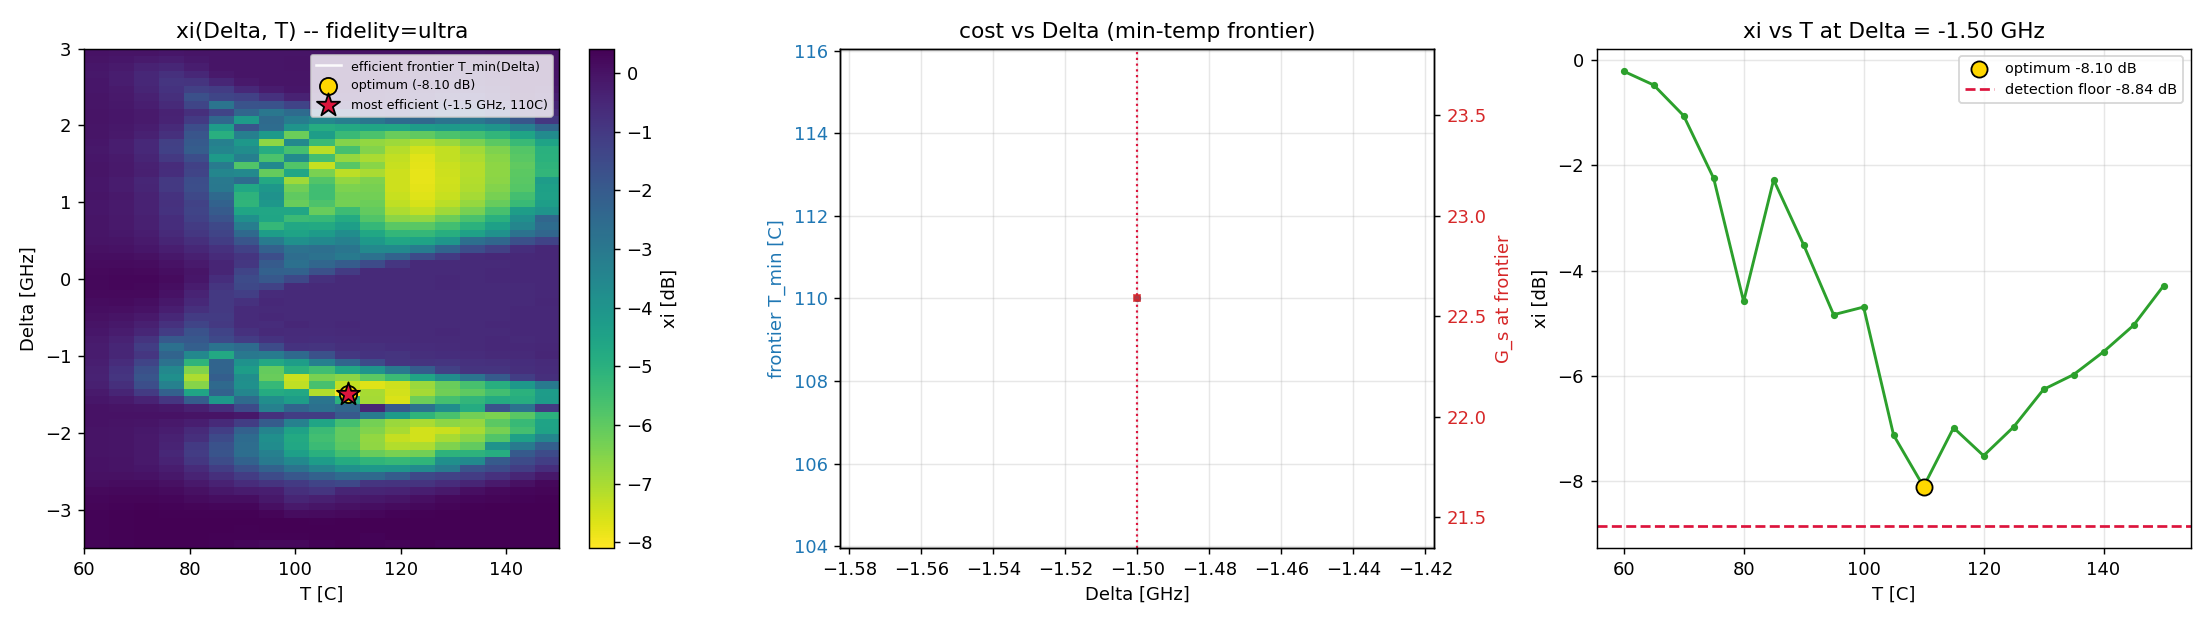
\includegraphics[width=\textwidth]{squeezing_frontier_v6.png}
\caption{v6 finite-loss hardened Ultra frontier. 최적점은
$\Delta=-1.50\GHz$, $T=110\degC$이다.}
\label{fig:v6frontier}
\end{figure}

\begin{table}[t]
\centering
\caption{v6 finite-loss hardened Ultra 주요 좌표. ``Sim default''는
$\Delta=+0.90\GHz$, $T=121\degC$, $\delta=-8\MHz$의 고정 readout이고,
나머지 frontier 행은 각 $(\Delta,T)$에서 $\delta$를 최적화한 값이다.}
\label{tab:finite}
\small
\setlength{\tabcolsep}{3pt}
\begin{tabularx}{\textwidth}{>{\raggedright\arraybackslash}Xrrrrrr}
\toprule
좌표 & $\Delta$ [GHz] & $T$ [$^\circ$C] & $\delta$ [MHz] &
$\xi$ [dB] & $G_s$ & $G_s-G_c$\\
\midrule
v6 전역 최적 & $-1.50$ & $110$ & $-280.0$ & $-8.102$ & $22.6$ & $0.623$\\
v6 최선 양(+)측 lobe & $+1.40$ & $125$ & $0.0$ & $-7.780$ & $39.0$ & $0.704$\\
Sim default readout & $+0.90$ & $121$ & $-8.0$ & $-7.203$ & $14.0$ & $0.904$\\
v5 최적 좌표 재평가 & $-2.00$ & $120$ & $-280.0$ & $-7.002$ & $7.0$ & $0.846$\\
v4 아티팩트 좌표 재평가 & $-2.20$ & $135$ & $-297.5$ & $-6.054$ & $28.8$ & $0.731$\\
\bottomrule
\end{tabularx}
\end{table}

v5에서 핵심이었던 $-2.0\GHz/120\degC$ 좌표는 beat 부호 교정 후 더 이상
frontier 최적이 아니다. gain이 $G_s\simeq27$에서 $G_s\simeq7$로 낮아지고,
스퀴징도 $-8.07\dB$에서 $-7.00\dB$ 수준으로 얕아진다. 반면 새 최적점
$-1.50\GHz/110\degC$는 중간 정도의 gain($G_s\simeq23$)과 낮은 in-cell
OD($0.024$)에서 finite-loss floor에 더 가깝게 접근한다. 양(+)측 lobe는
여전히 근접하지만 $0.32\dB$ 얕다.

\begin{figure}[t]
\centering
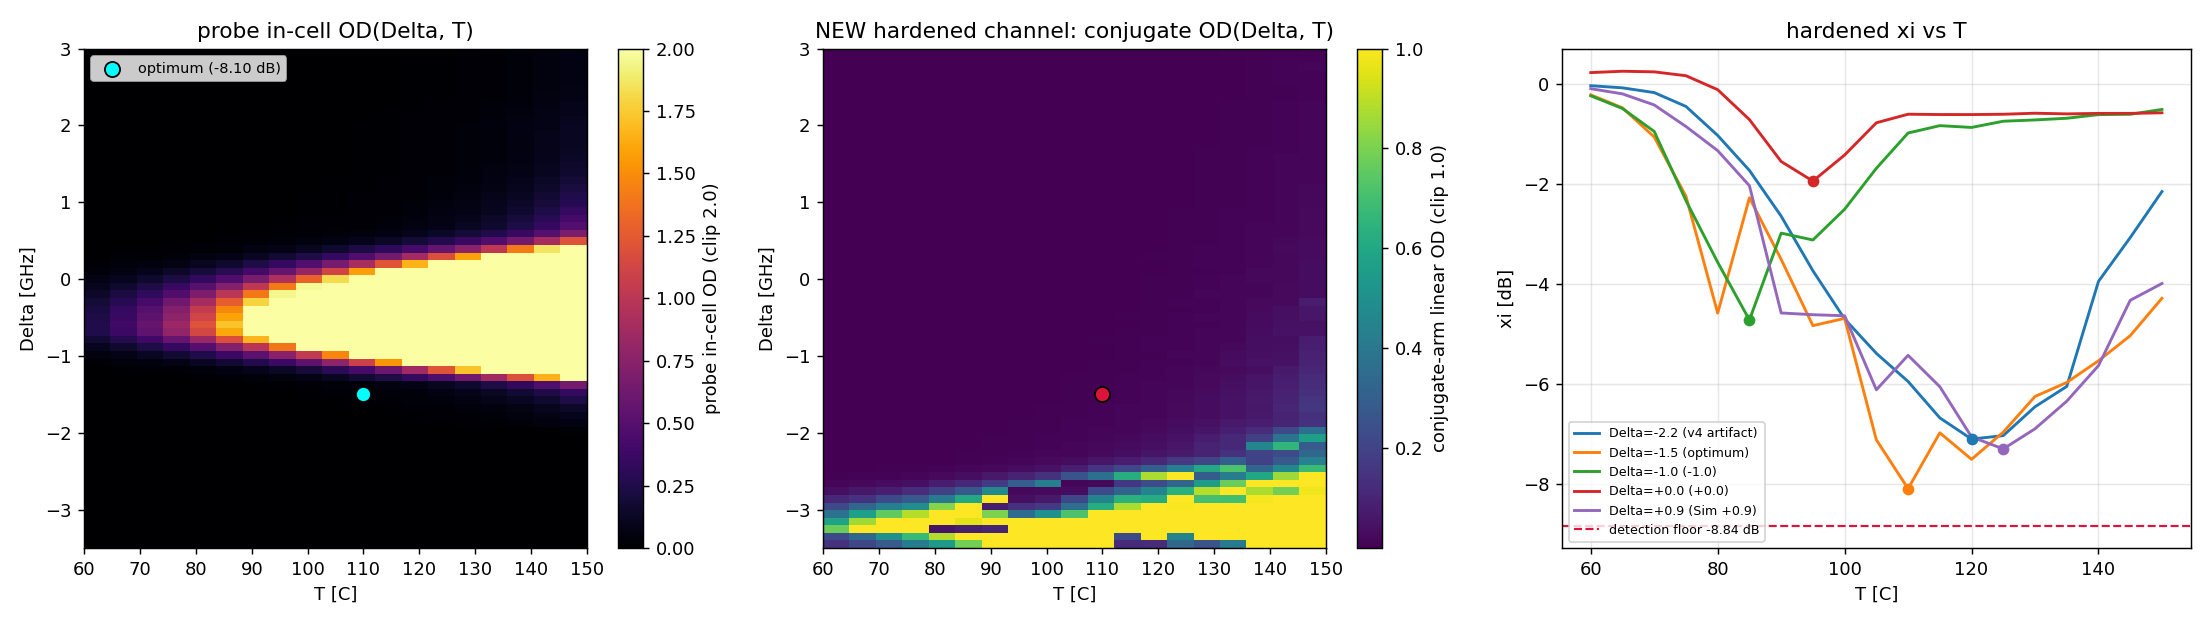
\includegraphics[width=\textwidth]{squeezing_frontier_od_v6.png}
\caption{v6 finite-loss OD 진단. 왼쪽은 probe in-cell OD, 가운데는 hardened
channel로 추가된 conjugate-arm linear OD, 오른쪽은 대표 detuning slice의
$\xi(T)$.}
\label{fig:v6od}
\end{figure}

\section{Ideal detection source-limit}

동일한 solve 격자를 $\eta=1$로 재사상한 ideal detection scan에서도 default
geometry 최적점은 같은 위치에 남는다:
\[
  \Delta=-1.50\GHz,\quad T=110\degC,\quad \delta\simeq-280\MHz,\quad
  \xi=-15.62\dB .
\]
검출 floor를 제거하면 깊이는 약 $7.5\dB$ 좋아지지만 최적 위치는 finite-loss와
같다.

\begin{figure}[t]
\centering
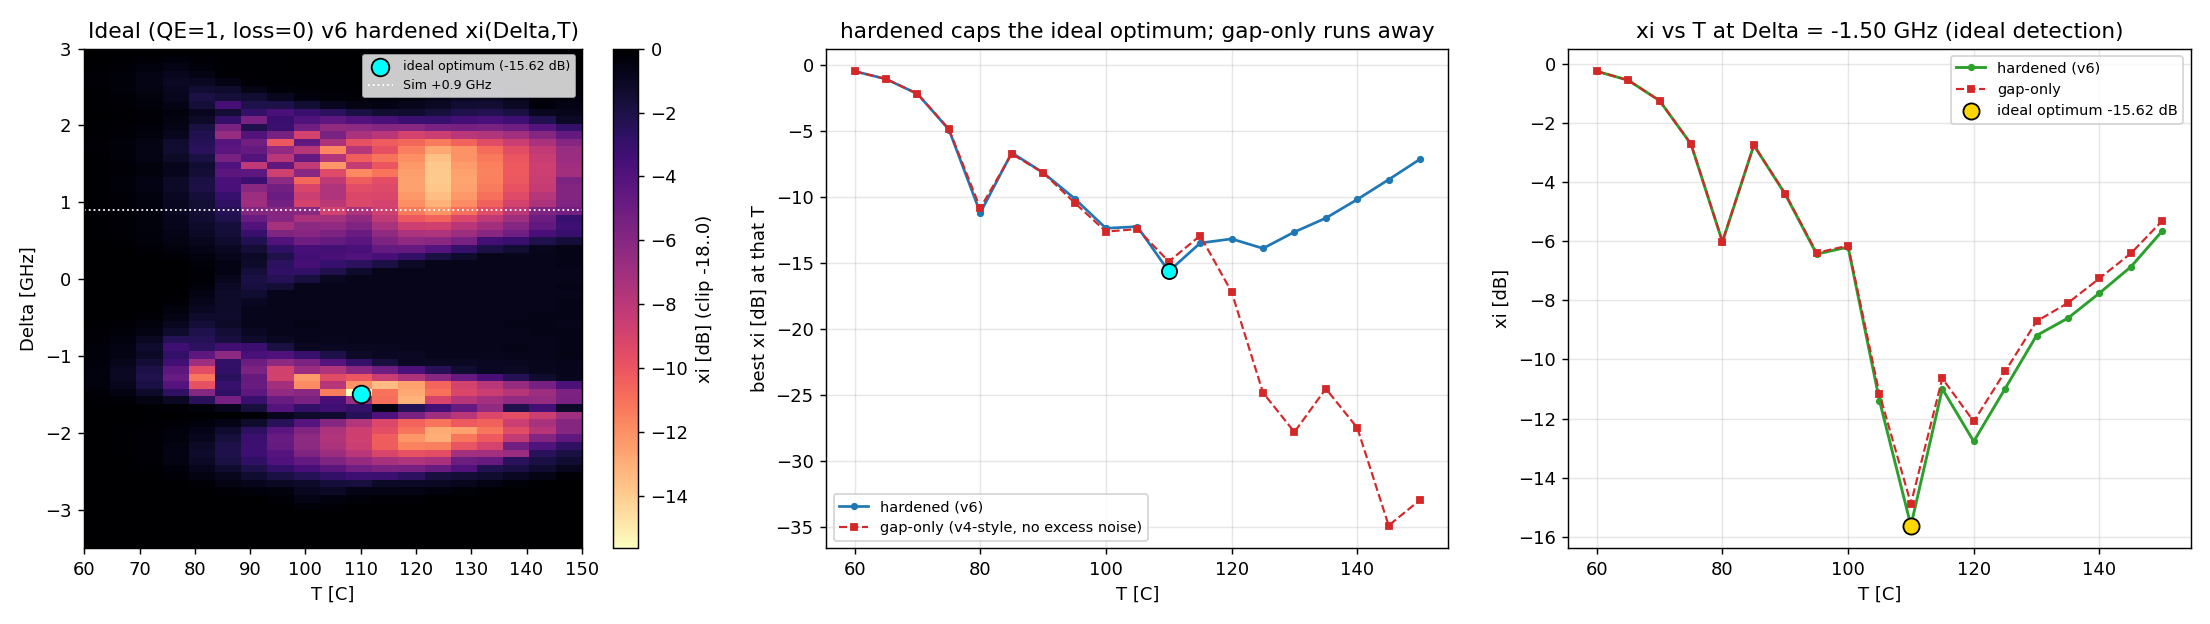
\includegraphics[width=\textwidth]{squeezing_frontier_ideal_qe1_v6.png}
\caption{v6 ideal detection($\eta=1$) hardened source-limit. gap-only 목적함수는
고이득 좌표로 폭주하지만, hardened channel은 그 좌표를 강하게 억제한다.}
\label{fig:v6ideal}
\end{figure}

\begin{table}[t]
\centering
\caption{v6 ideal detection 주요 좌표.}
\label{tab:ideal}
\small
\setlength{\tabcolsep}{3pt}
\begin{tabularx}{\textwidth}{>{\raggedright\arraybackslash}Xrrrrrr}
\toprule
좌표 & $\Delta$ [GHz] & $T$ [$^\circ$C] & $\delta$ [MHz] &
$\xi$ [dB] & $G_s$ & 비고\\
\midrule
v6 ideal 전역 최적 & $-1.50$ & $110$ & $-280.0$ & $-15.621$ & $22.6$ & default geometry\\
v6 ideal 최선 양(+)측 & $+1.30$ & $125$ & $0.0$ & $-13.883$ & $40.7$ & $1.74\dB$ 얕음\\
Sim default readout & $+0.90$ & $121$ & $-8.0$ & $-11.757$ & $14.0$ & fixed readout\\
v5 최적 좌표 재평가 & $-2.00$ & $120$ & $-280.0$ & $-11.086$ & $7.0$ & 더 이상 최적 아님\\
gap-only runaway & $-2.20$ & $145$ & $-87.5$ & $-34.889$ & $1416$ & hardened에서는 $-3.933\dB$\\
\bottomrule
\end{tabularx}
\end{table}

이상 검출 결과는 두 가지를 동시에 보여준다. v5의 핵심 주장 중
``gap-only 고이득 아티팩트는 hardened model로 제거된다''는 부분은 그대로
유효하다. 그러나 ``$-2.0\GHz/120\degC$가 남는 최적점''이라는 위치 해석은
v6에서 폐기된다. 새 위치는 더 낮은 온도와 덜 먼 red detuning 쪽이다.

\section{TPD/angle 상세 스캔}
\label{sec:tpdangle}

v6 ideal default optimum 주변에서 TPD와 pump--probe angle을 명시적으로
스캔했다. 기본 상세 스캔은
\[
  \Delta\in[-1.56,-1.44]\GHz,\quad
  T\in[96,114]\degC,\quad
  \theta\in[0,0.36]^\circ,\quad
  \delta\in[-420,-160]\MHz
\]
를 사용했다. v5와 같은 gate, $0.5\le G_s-G_c\le1.5$와 TPD-edge 제외를
적용했다.

\begin{figure}[p]
\centering
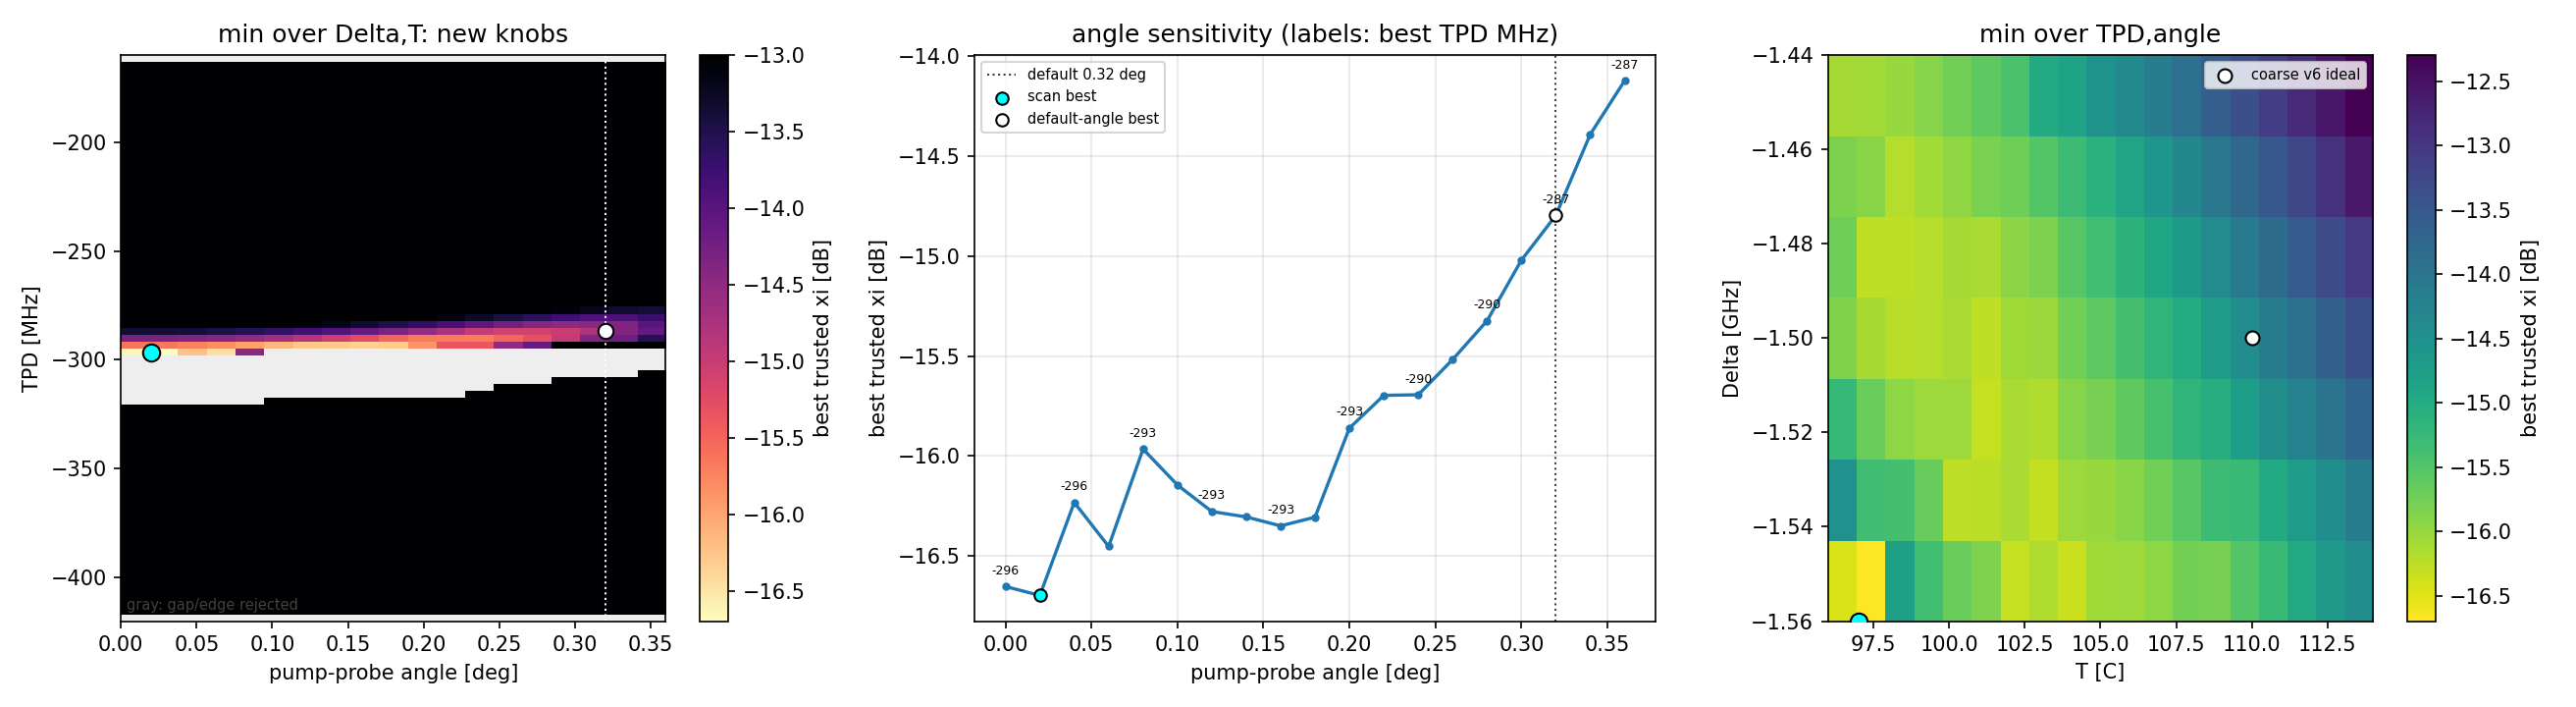
\includegraphics[width=\textwidth]{squeezing_frontier_ideal_v6_tpd_angle_detail.png}
\caption{v6 ideal 상세 TPD/angle scan. 흰 점은 기본 $0.32^\circ$ geometry의
상세 최적, 청록 점은 해당 local scan의 trusted 최저점이다.}
\label{fig:v6tpd}
\end{figure}

\begin{table}[t]
\centering
\caption{v6 TPD/angle 상세 및 low-angle 보조 스캔.}
\label{tab:detail}
\small
\setlength{\tabcolsep}{3pt}
\begin{tabularx}{\textwidth}{>{\raggedright\arraybackslash}Xrrrrrr>{\raggedright\arraybackslash}X}
\toprule
좌표 & $\Delta$ [GHz] & $T$ [$^\circ$C] & $\theta$ [$^\circ$] &
$\delta$ [MHz] & $\xi$ [dB] & $G_s-G_c$ & 비고\\
\midrule
coarse ideal frontier & $-1.50$ & $110$ & $0.32$ & $-280.0$ & $-15.62$ & $0.623$ & full-grid remap\\
상세, 기본 angle & $-1.54$ & $106$ & $0.32$ & $-286.8$ & $-14.80$ & $0.511$ & fixed geometry\\
상세 local 4D best & $-1.56$ & $97$ & $0.02$ & $-296.5$ & $-16.70$ & $0.500$ & low-angle edge\\
보조 low-angle trusted & $-1.66$ & $102$ & $0.02$ & $-307.0$ & $-20.70$ & $0.501$ & ridge 진단값\\
보조 raw no-gap & $-1.68$ & $88$ & $0.20$ & $-304.7$ & $-27.59$ & $-0.013$ & gate 실패\\
\bottomrule
\end{tabularx}
\end{table}

\begin{figure}[p]
\centering
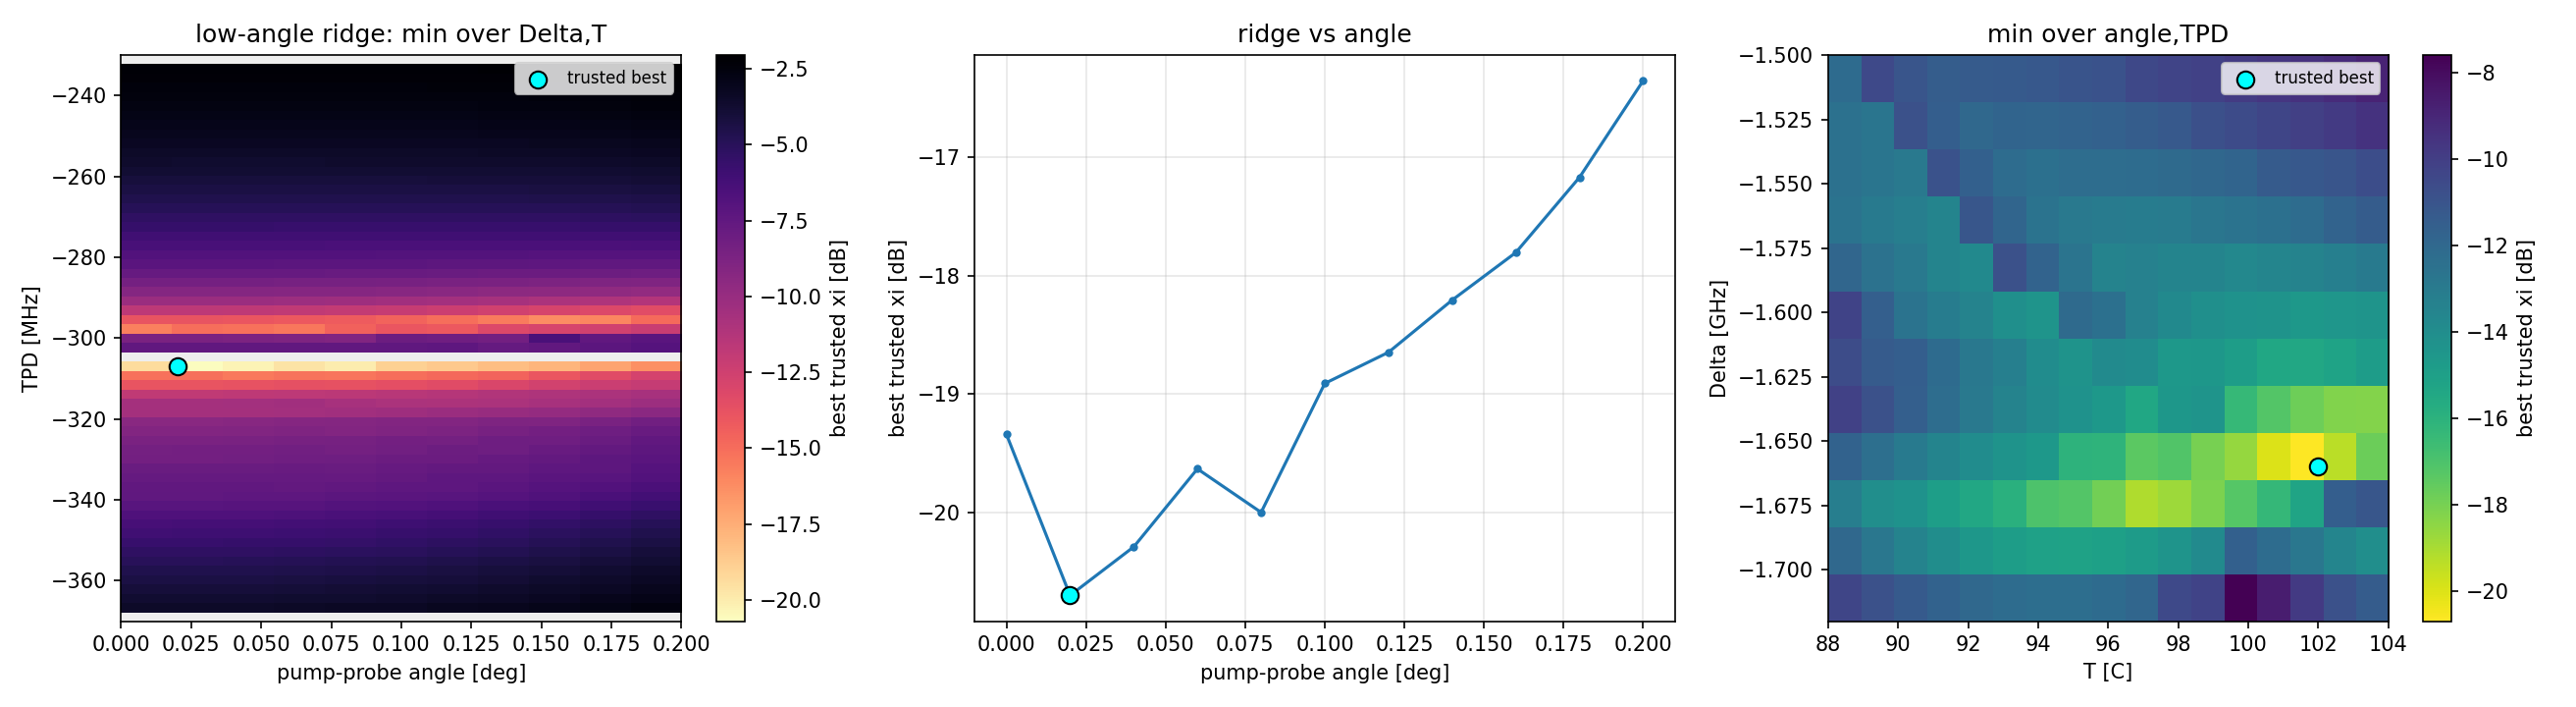
\includegraphics[width=\textwidth]{squeezing_frontier_ideal_v6_low_angle_ridge.png}
\caption{v6 low-angle ridge 보조 스캔. trusted best는
$\theta=0.02^\circ$에서 나타나며, raw best는 $G_s-G_c$ gate를 통과하지 못한다.}
\label{fig:v6ridge}
\end{figure}

기본 $0.32^\circ$ geometry 안에서는 source-limit이 대략 $-15\dB$ 정도로
정리된다. 그러나 angle을 거의 0으로 낮추면 phase mismatch와 spatial-overlap
penalty가 동시에 완화되어 훨씬 깊은 ridge가 열린다. 이 ridge는 real experiment의
beam separation, spatial filtering, pump leakage, EOM leakage, phase matching
calibration에 민감하므로 default geometry frontier의 즉시 대체 최적점으로 쓰면
안 된다. v6에서 더 정직한 표현은 다음과 같다.
\[
  \text{default geometry optimum: } -8.10\dB\ {\rm (finite)},\quad
  -15.62\dB\ {\rm (ideal)}
\]
이며, low-angle ridge는 별도의 geometry-calibration target이다.

\section{해석}

v6의 결론은 v5의 일부를 유지하고 일부를 교체한다.

\begin{enumerate}[leftmargin=1.5em]
\item \textbf{유지되는 부분: hardened model의 역할.}
      conjugate/probe linear OD와 pump scatter를 넣으면 gap-only 목적함수의
      고이득 폭주가 제거된다. ideal scan의 gap-only best는 $G_s\simeq1416$,
      $\xi=-34.89\dB$까지 폭주하지만, 같은 좌표의 hardened readout은
      $-3.93\dB$로 억제된다.
\item \textbf{교체되는 부분: v5의 $-2.0\GHz/120\degC$ 최적점.}
      beat 부호 교정 후 이 좌표는 finite-loss에서 $-7.00\dB$에 그친다.
      새 default-geometry 최적점은 $-1.50\GHz/110\degC$이다.
\item \textbf{남는 부분: 음(-)측 선호.}
      양(+)측 lobe와의 차이는 finite-loss에서 $0.32\dB$, ideal에서
      $1.74\dB$이다. 즉 음(-)측 선호는 사라지지 않지만, v5보다 더
      낮은 온도/낮은 OD/중간 gain의 optimum으로 재해석된다.
\item \textbf{새로운 분리: default geometry와 low-angle ridge.}
      low-angle ridge는 숫자로는 매력적이지만, 현재 모델의 geometry
      calibration 범위를 넘어서는 진단값이다. 실험 설계에는 기본
      $0.32^\circ$ 결과와 low-angle 가능성을 분리해서 써야 한다.
\end{enumerate}

\section{재현 명령}

\begin{itemize}[leftmargin=1.5em]
\item finite-loss v6 frontier:
\begin{verbatim}
python .claude/skills/fwm-squeezing-frontier/scripts/scan_squeezing_frontier.py \
  --fidelity ultra --out analysis/squeezing_frontier_finite_loss_v6
\end{verbatim}
\item ideal detection v6 frontier:
\begin{verbatim}
python .claude/skills/fwm-squeezing-frontier/scripts/scan_squeezing_frontier.py \
  --fidelity ultra --qe 1 --loss 0 --out analysis/squeezing_frontier_ideal_v6
\end{verbatim}
\item v6 report figures:
\begin{verbatim}
python docs/squeezing_report/make_v6_hardened_figs.py
python docs/squeezing_report/make_v6_ideal_figs.py
\end{verbatim}
\item v6 TPD/angle detail:
\begin{verbatim}
python analysis/scan_squeezing_v6_loss0_tpd_angle_detail.py
\end{verbatim}
\item full test suite after the beat-sign correction:
\begin{verbatim}
python -m pytest -q
\end{verbatim}
\end{itemize}

\noindent
\textbf{한 줄 요약.}
\emph{seeded beat 부호를 고친 v6에서 v5의 far-red optimum은
$-1.50\GHz/110\degC$로 이동한다. 음(-)측 선호는 남지만, 그 물리적 해석은
더 낮은 온도와 중간 gain의 default-geometry optimum으로 바뀌며, 거의 0도에
가까운 low-angle ridge는 별도 geometry-calibration 문제로 분리해야 한다.}

\end{document}
